% -------------------------------------------------
% فصل 4
% -------------------------------------------------

\projectchapter{پیاده‌سازی و نتایج}{
در این فصل، نحوه پیاده‌سازی مسیرهای طبقه‌بندی و خوشه‌بندی برای دو مجموعه‌داده مستقل متن و گفتار ارائه می‌شود. تمام نتایج گزارش‌شده از اجرای نهایی پروژه و مصنوعات ذخیره‌شده آن استخراج شده‌اند. مدل منتخب متن، \lr{Logistic Regression}، به دقت 0.9953 و مدل منتخب گفتار، \lr{KNN}، به دقت 0.9932 روی آزمون نهایی رسیده‌اند. خوشه‌بندی متن جدایی بسیار قوی زبان‌ها را نشان داد، اما در خوشه‌بندی گفتار بهترین ساختار داخلی الزاماً با زبان واقعی منطبق نبود. برای انتخاب طبقه‌بندها از میانگین \lr{Macro F1} در اعتبارسنجی متقاطع گروه‌آگاه روی داده آموزشی استفاده شده و مجموعه آزمون نهایی در تنظیم ابرپارامتر یا انتخاب مدل نقشی نداشته است. در خوشه‌بندی نیز برچسب زبان هنگام برازش و انتخاب پارامترها استفاده نشده و معیارهای خارجی تنها پس از تشکیل خوشه‌ها محاسبه شده‌اند.
}


% =================================================
\section{پیاده‌سازی بخش شناسایی زبان از متن}
% =================================================

ورودی مسیر طبقه‌بندی متن، متن خام یونیکد است. هر مدل به‌صورت یک خط لوله کامل پیاده‌سازی شده است تا پاک‌سازی، استخراج ویژگی، انتخاب ویژگی و طبقه‌بندی در یک زنجیره واحد قرار گیرند. ترتیب مراحل خط لوله به صورت زیر است:

\begin{center}
\lr{Raw Text}
$\longrightarrow$
\lr{Whitespace Cleaning}
$\longrightarrow$
\lr{Character/Word TF-IDF}
$\longrightarrow$
\lr{Chi-Square Top-50}
$\longrightarrow$
\lr{Classifier}
\end{center}

ویژگی‌های کاراکتری از
\lr{Character N-Gram}
های 2 تا 4 و ویژگی‌های واژگانی از
\lr{Word N-Gram}
های 1 تا 2 تشکیل شده‌اند. سقف تعداد ویژگی‌های دو بردارساز به‌ترتیب 3000 و 2000 است. انتخاب 50 ویژگی برتر با معیار
\lr{Chi-Square}
انجام می‌شود.

برای جلوگیری از نشت اطلاعات، تمام این مراحل داخل خط لوله مدل قرار دارند. بنابراین در هر دور اعتبارسنجی، بردارسازهای
\lr{TF-IDF}
و انتخاب‌گر ویژگی فقط روی بخش آموزشی همان دور برازش می‌شوند.

از مجموع 608 نمونه متنی، 397 نمونه برای آموزش و 211 نمونه برای آزمون نهایی استفاده شده‌اند. تقسیم داده با روش
\lr{Stratified Group K-Fold}
و با ثابت تصادفی 42 انجام شده است. گروه‌های مربوط به یک گوینده یا منبع در دو بخش آموزش و آزمون هم‌پوشانی ندارند. برای تنظیم مدل‌های متن نیز اعتبارسنجی متقاطع گروه‌آگاه پنج‌قسمتی روی بخش آموزشی اجرا شده است.

معیار اصلی انتخاب مدل
\lr{Macro F1}
است؛ زیرا این معیار عملکرد تمام زبان‌ها را با وزن برابر در نظر می‌گیرد. در کنار آن،
\lr{Accuracy}،
\lr{Precision}،
\lr{Recall}،
\lr{Weighted F1}
و ماتریس درهم‌ریختگی نیز برای مجموعه آزمون گزارش شده‌اند.


% =================================================
\section{طبقه‌بندی داده‌های متنی}
% =================================================

چهار خانواده مستقل برای طبقه‌بندی متن اجرا شده‌اند:

\begin{itemize}
	\item \lr{K-Nearest Neighbors}؛
	\item \lr{Decision Tree}؛
	\item \lr{Logistic Regression}؛
	\item \lr{Multinomial Naive Bayes}.
\end{itemize}

برای هر خانواده، شبکه ابرپارامتر از پیش تعریف شده و با
\lr{GridSearchCV}
بررسی شده است. فضای جست‌وجو و بهترین تنظیم انتخاب‌شده در جدول
\ref{tab:text-classifier-search}
ارائه شده‌اند.

\begin{table}[H]
\centering
\caption{فضای جست‌وجو و بهترین ابرپارامترهای طبقه‌بندهای متن}
\label{tab:text-classifier-search}
\small
\resizebox{\textwidth}{!}{%
\begin{tabular}{l l l}
\toprule
\textbf{مدل} & \textbf{فضای جست‌وجو} & \textbf{بهترین تنظیم} \\
\midrule
\lr{KNN} &
\lr{n\_neighbors: [1,3,5,10,20,30,50,75,100,150,200,250]} &
\lr{n\_neighbors=1, metric=cosine, weights=uniform} \\

\lr{Decision Tree} &
\lr{max\_depth: [1,2,3,4,5,6,7,8,10,12,15,20]} &
\lr{max\_depth=10} \\

\lr{Logistic Regression} &
\lr{C: [0.0001,0.001,0.01,0.1,0.5,1,2,5,10,50,100]} &
\lr{C=100, class\_weight=balanced} \\

\lr{Multinomial NB} &
\lr{alpha: [0.001,0.01,0.1,0.5,1,2,5,10,20,50,100,200]} &
\lr{alpha=0.001} \\
\bottomrule
\end{tabular}%
}
\end{table}

نتایج مقایسه چهار مدل در جدول
\ref{tab:text-classification-results}
آمده است. مقدار
\lr{CV Macro F1}
میانگین پنج دور اعتبارسنجی گروه‌آگاه روی بخش آموزشی است و ستون‌های آزمون فقط عملکرد نهایی روی 211 نمونه نگه‌داشته‌شده را نشان می‌دهند.

\begin{table}[H]
\centering
\caption{مقایسه نتایج طبقه‌بندی متن}
\label{tab:text-classification-results}
\small
\resizebox{\textwidth}{!}{%
\begin{tabular}{l c c c c c c c}
\toprule
\textbf{مدل} &
\textbf{\lr{CV Macro F1}} &
\textbf{انحراف معیار} &
\textbf{\lr{Accuracy}} &
\textbf{\lr{Macro Precision}} &
\textbf{\lr{Macro Recall}} &
\textbf{\lr{Macro F1}} &
\textbf{\lr{Weighted F1}} \\
\midrule
\lr{Logistic Regression} & 0.9906 & 0.0050 & 0.9953 & 0.9949 & 0.9944 & 0.9946 & 0.9953 \\
\lr{KNN}                 & 0.9770 & 0.0150 & 0.9858 & 0.9851 & 0.9840 & 0.9843 & 0.9858 \\
\lr{Decision Tree}       & 0.9537 & 0.0298 & 0.9858 & 0.9842 & 0.9837 & 0.9838 & 0.9858 \\
\lr{Multinomial NB}      & 0.8813 & 0.1213 & 0.9810 & 0.9777 & 0.9792 & 0.9773 & 0.9807 \\
\bottomrule
\end{tabular}%
}
\end{table}

براساس معیار از پیش تعیین‌شده،
\lr{Logistic Regression}
با میانگین
\lr{CV Macro F1}
برابر 0.9906 به‌عنوان مدل منتخب متن ذخیره شده است. این مدل روی مجموعه آزمون به دقت 0.9953 و
\lr{Macro F1}
برابر 0.9946 رسید و فقط یک نمونه از زبان اسپانیایی را پرتغالی پیش‌بینی کرد.

درخت تصمیم روی داده آموزشی به دقت 1.0 رسید، اما میانگین
\lr{Macro F1}
اعتبارسنجی آن 0.9537 بود. این اختلاف نشان می‌دهد که نتیجه کامل روی داده آموزشی به‌تنهایی معیار مناسبی برای انتخاب مدل نیست. همچنین
\lr{Multinomial Naive Bayes}
با انحراف معیار 0.1213 بیشترین نوسان را میان دورهای اعتبارسنجی داشت.

گزارش کامل طبقه‌بندی مدل منتخب در جدول
\ref{tab:text-best-classification-report}
ارائه شده است.

\begin{table}[H]
\centering
\caption{گزارش طبقه‌بندی \lr{Logistic Regression} روی مجموعه آزمون متن}
\label{tab:text-best-classification-report}
\begin{tabular}{l c c c c}
\toprule
\textbf{کلاس} & \textbf{\lr{Precision}} & \textbf{\lr{Recall}} & \textbf{\lr{F1-Score}} & \textbf{\lr{Support}} \\
\midrule
\lr{german}      & 1.0000 & 1.0000 & 1.0000 & 52 \\
\lr{italian}     & 1.0000 & 1.0000 & 1.0000 & 26 \\
\lr{japanese}    & 1.0000 & 1.0000 & 1.0000 & 33 \\
\lr{korean}      & 1.0000 & 1.0000 & 1.0000 & 38 \\
\lr{portuguese}  & 0.9697 & 1.0000 & 0.9846 & 32 \\
\lr{spanish}     & 1.0000 & 0.9667 & 0.9831 & 30 \\
\midrule
\lr{Macro Avg}    & 0.9949 & 0.9944 & 0.9946 & 211 \\
\lr{Weighted Avg} & 0.9954 & 0.9953 & 0.9953 & 211 \\
\bottomrule
\end{tabular}
\end{table}

ماتریس درهم‌ریختگی شکل
\ref{fig:text-logistic-confusion}
نیز نشان می‌دهد که تنها خطای مدل میان دو زبان اسپانیایی و پرتغالی رخ داده است.

\begin{figure}[H]
\centering
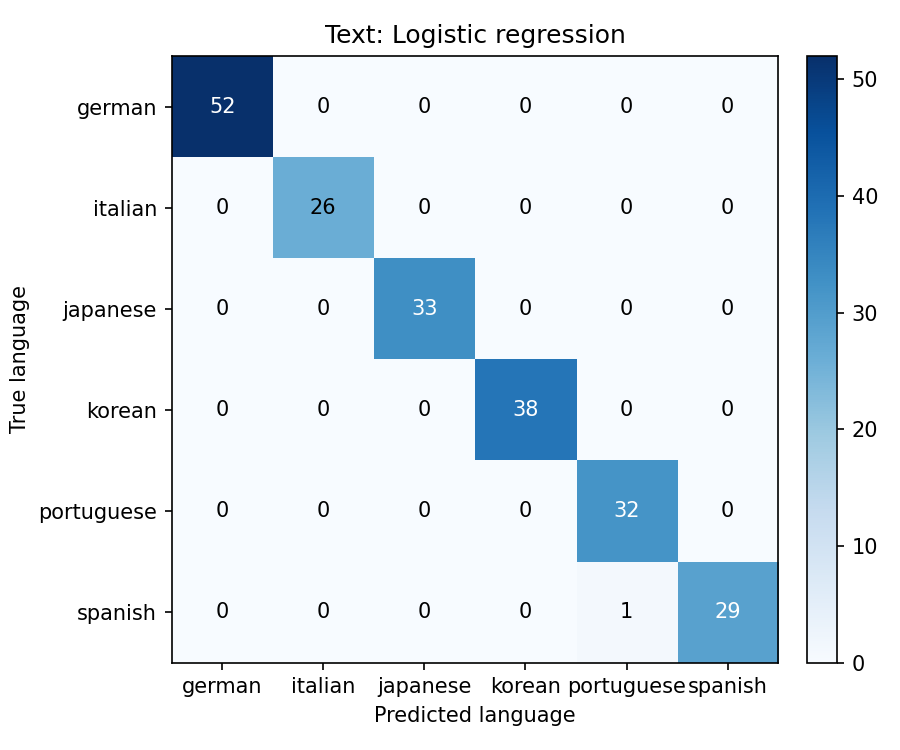
\includegraphics[width=0.88\textwidth]{../artifacts/text/classification/plots/logistic_regression_confusion_matrix.png}
\caption{ماتریس درهم‌ریختگی مدل منتخب طبقه‌بندی متن روی 211 نمونه آزمون}
\label{fig:text-logistic-confusion}
\end{figure}

گزارش طبقه‌بندی و ماتریس درهم‌ریختگی برای هر چهار مدل به‌صورت مستقل در پوشه مصنوعات بخش متن ذخیره شده‌اند. بسته نهایی استنتاج نیز کل زنجیره پاک‌سازی، بردارسازی، انتخاب ویژگی و مدل منتخب را در بر می‌گیرد و آزمون استنتاج مستقیم از متن خام را با موفقیت گذرانده است.


% =================================================
\section{خوشه‌بندی داده‌های متنی}
% =================================================

در مسیر خوشه‌بندی متن، استفاده از
\lr{Chi-Square}
مجاز نیست؛ زیرا این روش به برچسب زبان نیاز دارد. در نتیجه، 608 متن پس از پاک‌سازی با ترکیب ویژگی‌های کاراکتری و واژگانی
\lr{TF-IDF}
بردارسازی و سپس بدون استفاده از برچسب با
\lr{Truncated SVD}
به 50 مؤلفه کاهش یافته‌اند. نرمال‌سازی
\lr{L2}
آخرین مرحله ساخت نمایش خوشه‌بندی است.

چهار خانواده خوشه‌بندی
\lr{K-Means}،
\lr{Agglomerative Clustering}،
\lr{Gaussian Mixture}
و
\lr{DBSCAN}
اجرا شده‌اند. برای سه خانواده نخست، تعداد خوشه یا مؤلفه بین 2 تا 8 بررسی شده است. در
\lr{Agglomerative Clustering}
دو روش اتصال
\lr{Ward}
و
\lr{Average}
مقایسه شده‌اند. مدل
\lr{Gaussian Mixture}
با کوواریانس قطری و براساس کمترین
\lr{BIC}
انتخاب شده است. در
\lr{DBSCAN}
مقادیر
\lr{min\_samples}
برابر 5 و 10 و چهار صدک 0.70، 0.80، 0.90 و 0.95 فاصله همسایه‌ها برای تعیین
\lr{eps}
بررسی شده‌اند.

پارامترهای منتخب هر خانواده در جدول
\ref{tab:text-clustering-parameters}
نشان داده شده‌اند.

\begin{table}[H]
\centering
\caption{پارامترهای منتخب الگوریتم‌های خوشه‌بندی متن}
\label{tab:text-clustering-parameters}
\begin{tabular}{l l l}
\toprule
\textbf{الگوریتم} & \textbf{پارامترهای منتخب} & \textbf{معیار انتخاب} \\
\midrule
\lr{K-Means}       & \lr{n\_clusters=6, n\_init=20} & بیشترین \lr{Silhouette} \\
\lr{Agglomerative} & \lr{n\_clusters=6, linkage=ward} & بیشترین \lr{Silhouette} \\
\lr{Gaussian Mixture} & \lr{n\_components=8, covariance=diag} & کمترین \lr{BIC} \\
\lr{DBSCAN} & \lr{eps=0.6376, min\_samples=5} & بیشترین \lr{Silhouette} معتبر، سپس نویز کمتر \\
\bottomrule
\end{tabular}
\end{table}

برچسب‌های زبان در هیچ‌یک از مراحل ساخت ویژگی، کاهش ابعاد، برازش خوشه‌بند یا انتخاب پارامتر وارد نشده‌اند. پس از پایان برازش، برچسب‌ها فقط برای محاسبه
\lr{ARI}،
\lr{NMI}
و
\lr{Purity}
به کار رفته‌اند. برای
\lr{DBSCAN}،
معیارهای داخلی فقط روی نمونه‌های غیرنویز محاسبه شده‌اند، اما معیارهای خارجی همه تخصیص‌ها، از جمله برچسب نویز $-1$، را در نظر می‌گیرند. نتایج در جدول
\ref{tab:text-clustering-results}
ارائه شده‌اند.

\begin{table}[H]
\centering
\caption{مقایسه نتایج خوشه‌بندی متن}
\label{tab:text-clustering-results}
\small
\resizebox{\textwidth}{!}{%
\begin{tabular}{l c c c c c c c c}
\toprule
\textbf{مدل} & \textbf{تعداد خوشه} & \textbf{نرخ نویز} & \textbf{\lr{Silhouette}} & \textbf{\lr{CH}} & \textbf{\lr{DB}} & \textbf{\lr{ARI}} & \textbf{\lr{NMI}} & \textbf{\lr{Purity}} \\
\midrule
\lr{DBSCAN}          & 13 & 0.2352 & 0.4265 & 80.9701  & 1.0614 & 0.8089 & 0.8673 & 0.8882 \\
\lr{K-Means}         & 6  & 0.0000 & 0.3511 & 152.6121 & 1.4845 & 1.0000 & 1.0000 & 1.0000 \\
\lr{Agglomerative}   & 6  & 0.0000 & 0.3511 & 152.6121 & 1.4845 & 1.0000 & 1.0000 & 1.0000 \\
\lr{Gaussian Mixture}& 8  & 0.0000 & 0.2599 & 116.5118 & 1.7507 & 0.8942 & 0.9404 & 1.0000 \\
\bottomrule
\end{tabular}%
}
\end{table}

براساس معیار داخلی از پیش تعیین‌شده،
\lr{DBSCAN}
با
\lr{Silhouette}
برابر 0.4265 انتخاب شده است. بااین‌حال، این مدل 13 خوشه تشکیل داده و 143 نمونه، معادل 23.52 درصد داده‌ها، را نویز تشخیص داده است. در محاسبه
\lr{Silhouette}
برای
\lr{DBSCAN}،
نمونه‌های نویز کنار گذاشته می‌شوند؛ به همین دلیل، مقدار بالاتر این معیار الزاماً به معنی بازیابی بهتر زبان‌ها برای تمام نمونه‌ها نیست.

در مقابل،
\lr{K-Means}
و
\lr{Agglomerative Clustering}
هر دو بدون استفاده از برچسب، شش خوشه ایجاد کرده و پس از برازش به
\lr{ARI=1}،
\lr{NMI=1}
و
\lr{Purity=1}
رسیده‌اند. این نتیجه نشان می‌دهد که در نمایش متنی پروژه، شش زبان از نظر الگوهای کاراکتری و واژگانی به‌طور کامل از یکدیگر جدا شده‌اند.

شکل‌های
\ref{fig:text-kmeans-clusters}
و
\ref{fig:text-dbscan-clusters}
دو نوع رفتار متفاوت را در دو مؤلفه نخست نمایش بدون برچسب نشان می‌دهند. این شکل‌ها فقط تصویر دوبعدی نمایش هستند و تمام 50 مؤلفه در برازش خوشه‌بند استفاده شده‌اند.

\begin{figure}[H]
\centering
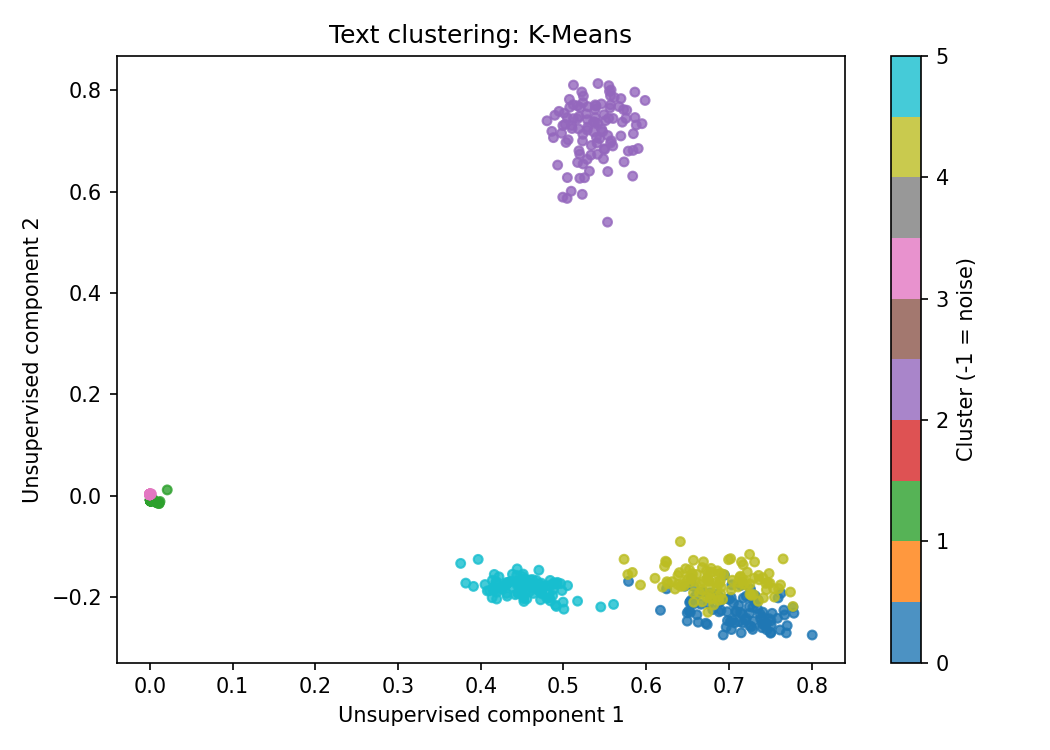
\includegraphics[width=0.82\textwidth]{../artifacts/text/clustering/plots/kmeans_clusters.png}
\caption{نمایش دوبعدی تخصیص خوشه‌های \lr{K-Means} برای داده‌های متنی}
\label{fig:text-kmeans-clusters}
\end{figure}

\begin{figure}[H]
\centering
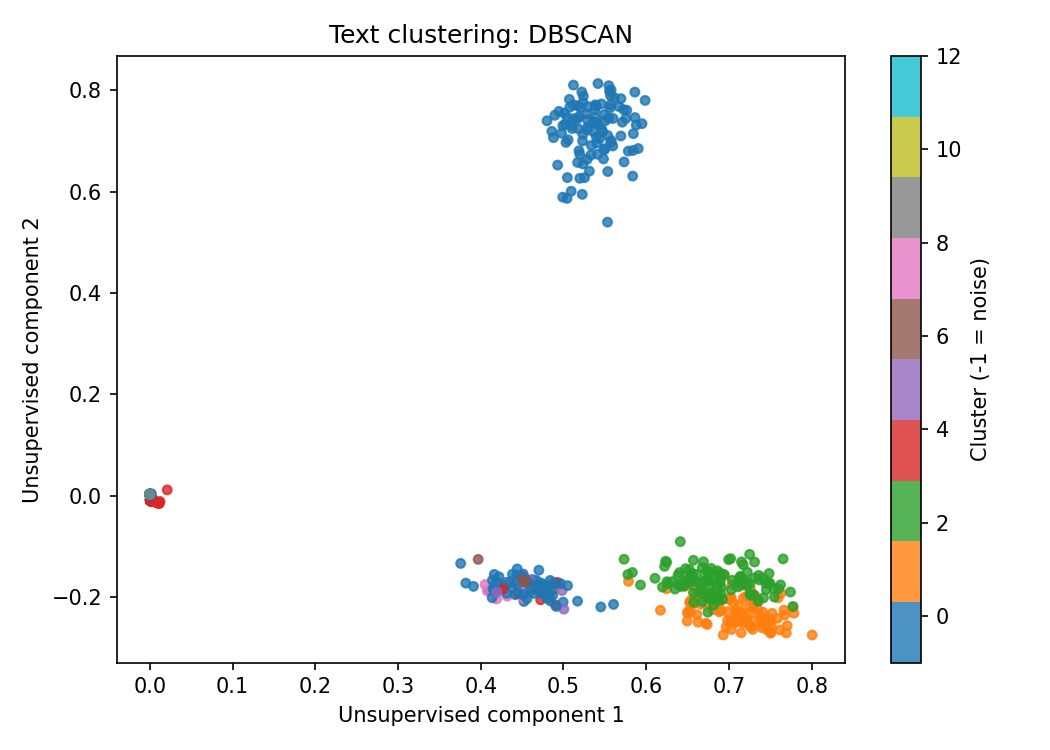
\includegraphics[width=0.82\textwidth]{../artifacts/text/clustering/plots/dbscan_clusters.png}
\caption{نمایش دوبعدی خوشه‌ها و نمونه‌های نویز \lr{DBSCAN} برای داده‌های متنی}
\label{fig:text-dbscan-clusters}
\end{figure}


% =================================================
\section{پیاده‌سازی بخش شناسایی زبان از گفتار}
% =================================================

پیاده‌سازی بخش گفتار از جدول
\lr{features.csv}
آغاز می‌شود که پیش‌تر توسط نگارنده از فایل‌های صوتی پاک‌سازی‌شده استخراج شده است. این جدول 720 سطر، سه ستون توصیفی و 133 ویژگی عددی دارد. ستون‌های
\lr{filepath}،
\lr{lang}
و
\lr{gender}
از ماتریس ورودی حذف می‌شوند؛ ستون
\lr{lang}
برچسب هدف است و جنسیت فقط برای توصیف داده نگهداری می‌شود.

فراداده با استفاده از مسیر پایدار فایل به جدول ویژگی متصل می‌شود و هم‌ترازی دو فایل به ترتیب سطرها وابسته نیست. در فایل نهایی هیچ مقدار گمشده یا بی‌نهایتی وجود ندارد؛ بااین‌حال، جایگزینی مقادیر گمشده با میانه به‌صورت دفاعی داخل خط لوله مدل‌ها حفظ شده است.

از 720 نمونه گفتاری، 572 نمونه برای آموزش و 148 نمونه برای آزمون نهایی در نظر گرفته شده‌اند. شناسه گوینده یا منبع از نام فایل استخراج شده و تقسیم با
\lr{Stratified Group K-Fold}
پنج‌قسمتی انجام شده است. هیچ گروه مشترکی میان مجموعه آموزش و آزمون وجود ندارد. برای تنظیم مدل‌های گفتار، اعتبارسنجی متقاطع گروه‌آگاه سه‌قسمتی فقط روی بخش آموزشی اجرا شده است.

در مدل‌های
\lr{Logistic Regression}،
\lr{RBF SVM}
و
\lr{KNN}،
جایگزینی میانه و استانداردسازی ویژگی‌ها پیش از طبقه‌بند قرار دارند. این مراحل در هر دور اعتبارسنجی فقط روی داده آموزشی برازش می‌شوند. برای
\lr{Random Forest}
استانداردسازی لازم نیست و تنها جایگزینی میانه در خط لوله قرار گرفته است.

برچسب‌های گفتار با یک رمزگذار برچسب که فقط روی داده آموزشی برازش شده است به مقادیر عددی تبدیل می‌شوند. مدل نهایی همراه با نام و ترتیب 133 ویژگی، رمزگذار برچسب و خط لوله پیش‌پردازش ذخیره شده است تا استنتاج روی یک سطر ویژگی جدید به‌صورت بازتولیدپذیر انجام شود.


% =================================================
\section{طبقه‌بندی گفتار}
% =================================================

چهار خانواده مستقل برای طبقه‌بندی ویژگی‌های گفتاری اجرا شده‌اند:

\begin{itemize}
	\item \lr{Logistic Regression}؛
	\item \lr{RBF Support Vector Machine}؛
	\item \lr{Random Forest}؛
	\item \lr{K-Nearest Neighbors}.
\end{itemize}

فضای جست‌وجو و بهترین ابرپارامترهای حاصل از اعتبارسنجی گروه‌آگاه در جدول
\ref{tab:speech-classifier-search}
ارائه شده‌اند.

\begin{table}[H]
\centering
\caption{فضای جست‌وجو و بهترین ابرپارامترهای طبقه‌بندهای گفتار}
\label{tab:speech-classifier-search}
\small
\resizebox{\textwidth}{!}{%
\begin{tabular}{l l l}
\toprule
\textbf{مدل} & \textbf{فضای جست‌وجو} & \textbf{بهترین تنظیم} \\
\midrule
\lr{Logistic Regression} &
\lr{C: [0.1,1,10],\ class\_weight: [None,balanced]} &
\lr{C=1,\ class\_weight=balanced} \\

\lr{RBF SVM} &
\lr{C: [1,10],\ gamma: [scale,0.01],\ class\_weight: [None,balanced]} &
\lr{C=1,\ gamma=scale,\ class\_weight=None} \\

\lr{Random Forest} &
\lr{n\_estimators=200,\ max\_depth: [None,12],\ min\_samples\_leaf: [1,2],\ class\_weight: [None,balanced]} &
\lr{200 trees,\ max\_depth=None,\ min\_samples\_leaf=1,\ class\_weight=balanced} \\

\lr{KNN} &
\lr{n\_neighbors: [3,7,11],\ weights: [uniform,distance],\ p: [1,2]} &
\lr{n\_neighbors=3,\ weights=uniform,\ p=1} \\
\bottomrule
\end{tabular}%
}
\end{table}

نتایج اعتبارسنجی و آزمون نهایی در جدول
\ref{tab:speech-classification-results}
نشان داده شده‌اند.

\begin{table}[H]
\centering
\caption{مقایسه نتایج طبقه‌بندی گفتار}
\label{tab:speech-classification-results}
\small
\resizebox{\textwidth}{!}{%
\begin{tabular}{l c c c c c c c}
\toprule
\textbf{مدل} &
\textbf{\lr{CV Macro F1}} &
\textbf{انحراف معیار} &
\textbf{\lr{Accuracy}} &
\textbf{\lr{Macro Precision}} &
\textbf{\lr{Macro Recall}} &
\textbf{\lr{Macro F1}} &
\textbf{\lr{Weighted F1}} \\
\midrule
\lr{KNN}                 & 0.9662 & 0.0444 & 0.9932 & 0.9891 & 0.9940 & 0.9914 & 0.9933 \\
\lr{Logistic Regression} & 0.9656 & 0.0486 & 1.0000 & 1.0000 & 1.0000 & 1.0000 & 1.0000 \\
\lr{Random Forest}       & 0.9544 & 0.0644 & 1.0000 & 1.0000 & 1.0000 & 1.0000 & 1.0000 \\
\lr{RBF SVM}             & 0.9246 & 0.0853 & 1.0000 & 1.0000 & 1.0000 & 1.0000 & 1.0000 \\
\bottomrule
\end{tabular}%
}
\end{table}

مدل
\lr{KNN}
با میانگین
\lr{CV Macro F1}
برابر 0.9662 بالاترین امتیاز اعتبارسنجی را به دست آورد و براساس قاعده از پیش تعیین‌شده به‌عنوان مدل منتخب ذخیره شد. این مدل روی 148 نمونه آزمون فقط یک نمونه آلمانی را کره‌ای پیش‌بینی کرد و به دقت 0.9932 و
\lr{Macro F1}
برابر 0.9914 رسید.

سه مدل
\lr{Logistic Regression}،
\lr{Random Forest}
و
\lr{RBF SVM}
روی مجموعه آزمون دقت 1.0 داشتند. بااین‌حال، این نتیجه برای انتخاب مدل استفاده نشده است؛ زیرا انتخاب مدل براساس آزمون نهایی باعث نشت تصمیم‌گیری به داده آزمون می‌شود. اختلاف میان امتیاز اعتبارسنجی
\lr{KNN}
و
\lr{Logistic Regression}
فقط حدود 0.0006 است و در مقایسه با انحراف معیار دورهای اعتبارسنجی بسیار کوچک محسوب می‌شود. بنابراین این دو مدل از نظر پایداری اعتبارسنجی بسیار نزدیک‌اند و نباید برتری قطعی
\lr{KNN}
را نتیجه گرفت.

گزارش طبقه‌بندی مدل منتخب گفتار در جدول
\ref{tab:speech-best-classification-report}
ارائه شده است.

\begin{table}[H]
\centering
\caption{گزارش طبقه‌بندی \lr{KNN} روی مجموعه آزمون گفتار}
\label{tab:speech-best-classification-report}
\begin{tabular}{l c c c c}
\toprule
\textbf{کلاس} & \textbf{\lr{Precision}} & \textbf{\lr{Recall}} & \textbf{\lr{F1-Score}} & \textbf{\lr{Support}} \\
\midrule
\lr{de} & 1.0000 & 0.9762 & 0.9880 & 42 \\
\lr{es} & 1.0000 & 1.0000 & 1.0000 & 30 \\
\lr{it} & 1.0000 & 1.0000 & 1.0000 & 54 \\
\lr{ko} & 0.9565 & 1.0000 & 0.9778 & 22 \\
\midrule
\lr{Macro Avg}    & 0.9891 & 0.9940 & 0.9914 & 148 \\
\lr{Weighted Avg} & 0.9935 & 0.9932 & 0.9933 & 148 \\
\bottomrule
\end{tabular}
\end{table}

شکل
\ref{fig:speech-knn-confusion}
ماتریس درهم‌ریختگی مدل منتخب را نمایش می‌دهد.

\begin{figure}[H]
\centering
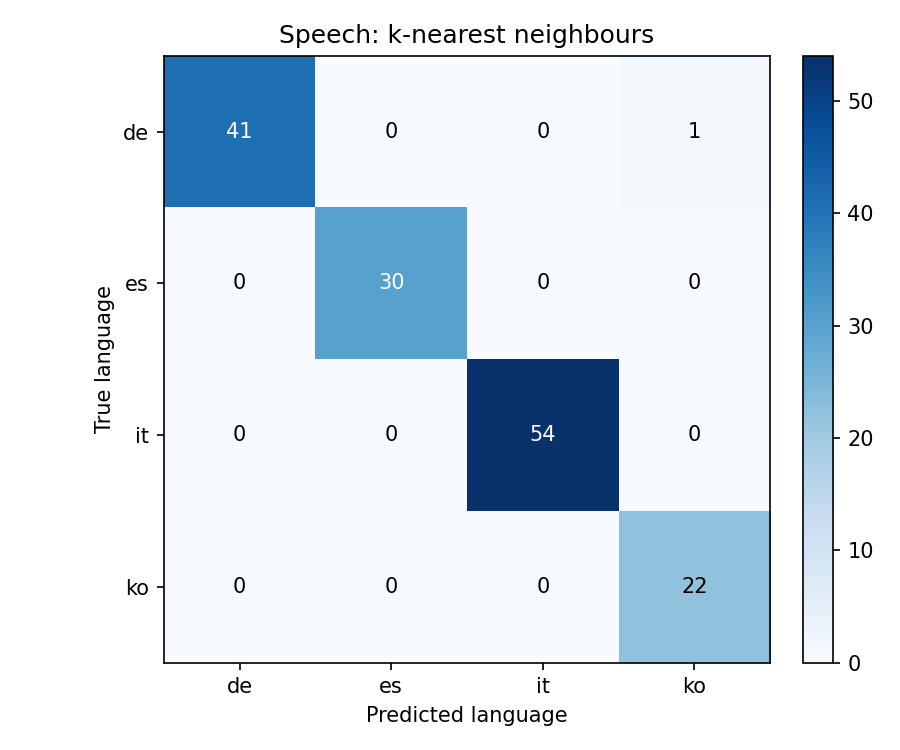
\includegraphics[width=0.82\textwidth]{../artifacts/speech/classification/plots/knn_confusion_matrix.png}
\caption{ماتریس درهم‌ریختگی مدل منتخب طبقه‌بندی گفتار روی 148 نمونه آزمون}
\label{fig:speech-knn-confusion}
\end{figure}

برای هر چهار مدل، فایل مدل، پیش‌بینی‌های آزمون، معیارهای عددی، گزارش طبقه‌بندی و ماتریس درهم‌ریختگی ذخیره شده‌اند. بسته استنتاج مدل منتخب نیز دریافت دقیق 133 ویژگی را کنترل می‌کند و آزمون استنتاج آن با موفقیت انجام شده است.

یک نکته اجرایی درباره فایل‌های
\lr{CSV}
پیش‌بینی گفتار وجود دارد: ستون
\lr{predicted\_language}
در این فایل‌ها با کد عددی رمزگذار ذخیره شده است؛ نگاشت آن برابر
\lr{0=de}،
\lr{1=es}،
\lr{2=it}
و
\lr{3=ko}
است. معیارها، گزارش‌های طبقه‌بندی و ماتریس‌های درهم‌ریختگی پیش از ذخیره این فایل و با نام زبان رمزگشایی‌شده محاسبه شده‌اند؛ بنابراین اعداد گزارش حاضر تحت تأثیر این قالب ذخیره‌سازی نیستند. بسته استنتاج نهایی نیز نام زبان را برمی‌گرداند.


% =================================================
\section{خوشه‌بندی گفتار}
% =================================================

برای خوشه‌بندی گفتار، هر 720 نمونه بدون استفاده از برچسب زبان وارد خط لوله‌ای شامل جایگزینی میانه، استانداردسازی و
\lr{PCA}
شده‌اند. تعداد مؤلفه‌های اصلی برابر 30 است. برچسب زبان نه در برازش این نمایش و نه در انتخاب پارامترهای خوشه‌بندی استفاده نشده است.

همان چهار خانواده خوشه‌بندی بخش متن روی نمایش گفتاری نیز اجرا شده‌اند. بازه تعداد خوشه یا مؤلفه 2 تا 8 بوده و قواعد انتخاب پارامترها با بخش متن یکسان هستند. پارامترهای منتخب در جدول
\ref{tab:speech-clustering-parameters}
ارائه شده‌اند.

\begin{table}[H]
\centering
\caption{پارامترهای منتخب الگوریتم‌های خوشه‌بندی گفتار}
\label{tab:speech-clustering-parameters}
\begin{tabular}{l l l}
\toprule
\textbf{الگوریتم} & \textbf{پارامترهای منتخب} & \textbf{معیار انتخاب} \\
\midrule
\lr{K-Means}       & \lr{n\_clusters=8,\ n\_init=20} & بیشترین \lr{Silhouette} \\
\lr{Agglomerative} & \lr{n\_clusters=2,\ linkage=average} & بیشترین \lr{Silhouette} \\
\lr{Gaussian Mixture} & \lr{n\_components=8,\ covariance=diag} & کمترین \lr{BIC} \\
\lr{DBSCAN} & \lr{eps=6.8887,\ min\_samples=5} & بیشترین \lr{Silhouette} معتبر، سپس نویز کمتر \\
\bottomrule
\end{tabular}
\end{table}

نتایج معیارهای داخلی و خارجی خوشه‌بندی گفتار در جدول
\ref{tab:speech-clustering-results}
آمده است.

\begin{table}[H]
\centering
\caption{مقایسه نتایج خوشه‌بندی گفتار}
\label{tab:speech-clustering-results}
\small
\resizebox{\textwidth}{!}{%
\begin{tabular}{l c c c c c c c c}
\toprule
\textbf{مدل} & \textbf{تعداد خوشه} & \textbf{نرخ نویز} & \textbf{\lr{Silhouette}} & \textbf{\lr{CH}} & \textbf{\lr{DB}} & \textbf{\lr{ARI}} & \textbf{\lr{NMI}} & \textbf{\lr{Purity}} \\
\midrule
\lr{Agglomerative}    & 2  & 0.0000 & 0.4709 & 5.8240   & 0.4037 & 0.0000 & 0.0028 & 0.2514 \\
\lr{DBSCAN}           & 13 & 0.1806 & 0.2963 & 71.8478  & 1.1705 & 0.2433 & 0.4696 & 0.7292 \\
\lr{K-Means}          & 8  & 0.0000 & 0.2382 & 100.8028 & 1.6214 & 0.4983 & 0.6731 & 0.9028 \\
\lr{Gaussian Mixture} & 8  & 0.0000 & 0.1499 & 67.1942  & 2.1394 & 0.3382 & 0.5402 & 0.8111 \\
\bottomrule
\end{tabular}%
}
\end{table}

اگر فقط معیار داخلی
\lr{Silhouette}
در نظر گرفته شود،
\lr{Agglomerative Clustering}
با مقدار 0.4709 انتخاب می‌شود. بااین‌حال، بررسی اندازه خوشه‌ها نشان داد که این مدل 719 نمونه را در یک خوشه و فقط یک نمونه را در خوشه دوم قرار داده است. در نتیجه،
\lr{ARI}
برابر صفر،
\lr{NMI}
تقریباً صفر و
\lr{Purity}
برابر 0.2514 است. بنابراین مقدار بالای
\lr{Silhouette}
در این حالت بیشتر حاصل جداسازی یک نمونه دورافتاده است و به معنای کشف زبان‌ها نیست.

در میان نتایج خارجی،
\lr{K-Means}
با
\lr{ARI=0.4983}،
\lr{NMI=0.6731}
و
\lr{Purity=0.9028}
بیشترین تطابق را با زبان‌ها دارد، هرچند به جای چهار خوشه، هشت خوشه ساخته است. این موضوع نشان می‌دهد که ساختار طبیعی ویژگی‌های صوتی احتمالاً علاوه بر زبان، تحت تأثیر عوامل دیگری مانند گوینده، شرایط ضبط یا ویژگی‌های آکوستیکی قرار دارد؛ تعیین سهم دقیق این عوامل به تحلیل جداگانه نیاز دارد.

مدل
\lr{DBSCAN}
نیز 13 خوشه ساخته و 130 نمونه، معادل 18.06 درصد داده‌ها، را نویز در نظر گرفته است. بنابراین در بخش گفتار هیچ‌یک از خوشه‌بندها زبان‌ها را به صورت چهار گروه مستقل و کامل بازیابی نکرده‌اند.

شکل
\ref{fig:speech-agglomerative-clusters}
رفتار نامتوازن مدل منتخب براساس
\lr{Silhouette}
را نشان می‌دهد. شکل
\ref{fig:speech-kmeans-clusters}
نیز تقسیم ریزتر داده توسط
\lr{K-Means}
را در دو مؤلفه نخست
\lr{PCA}
نمایش می‌دهد. هر دو شکل فقط فرافکنی دوبعدی هستند و خوشه‌بندی روی هر 30 مؤلفه انجام شده است.

\begin{figure}[H]
\centering
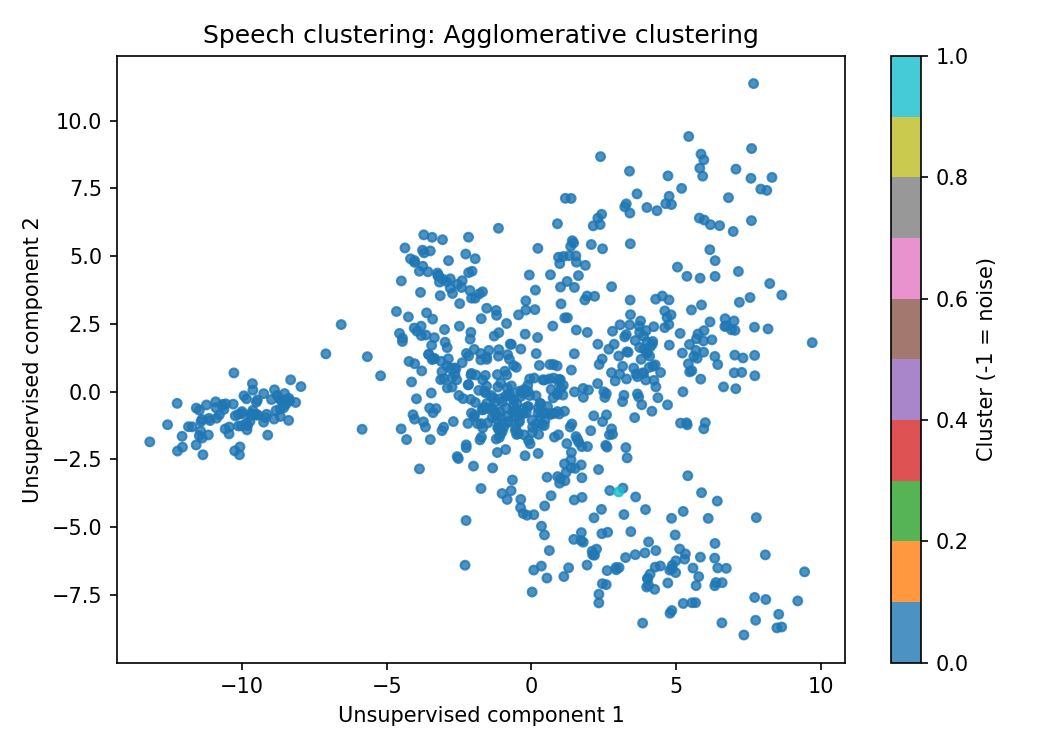
\includegraphics[width=0.82\textwidth]{../artifacts/speech/clustering/plots/agglomerative_clusters.png}
\caption{نمایش دوبعدی خوشه‌بندی سلسله‌مراتبی گفتار؛ یک خوشه شامل 719 نمونه و خوشه دیگر شامل یک نمونه است}
\label{fig:speech-agglomerative-clusters}
\end{figure}

\begin{figure}[H]
\centering
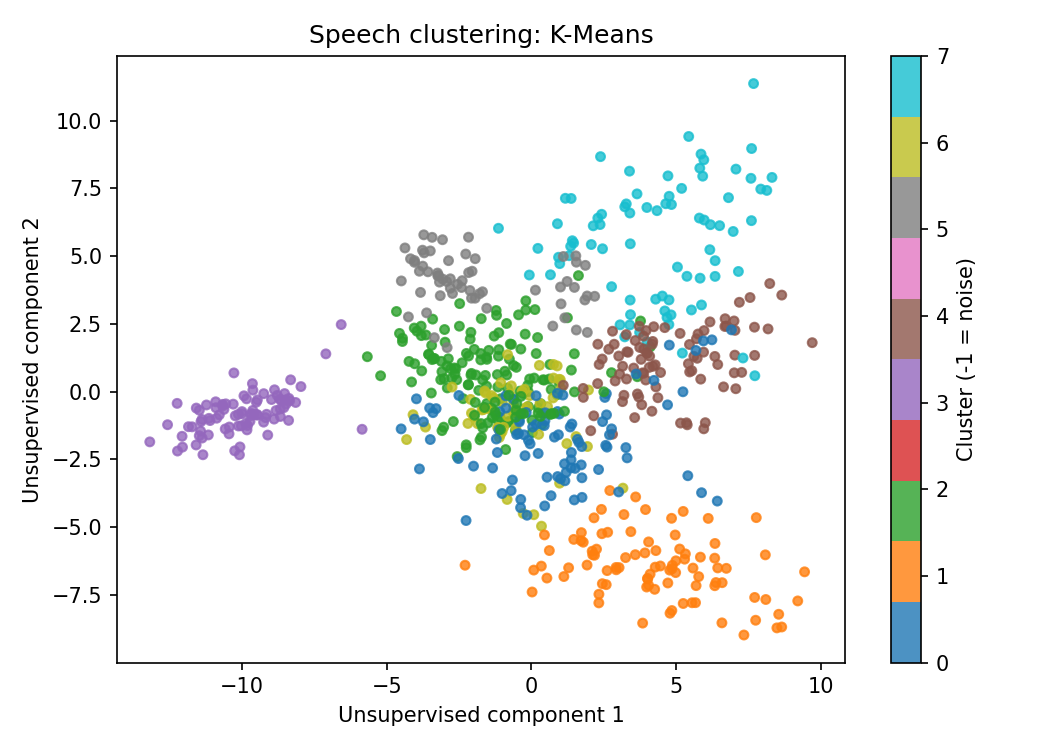
\includegraphics[width=0.82\textwidth]{../artifacts/speech/clustering/plots/kmeans_clusters.png}
\caption{نمایش دوبعدی هشت خوشه \lr{K-Means} برای ویژگی‌های گفتاری}
\label{fig:speech-kmeans-clusters}
\end{figure}


% =================================================
\section{ارزیابی و مقایسه نتایج}
% =================================================

جدول
\ref{tab:best-classifiers-summary}
خلاصه مدل منتخب هر مسیر طبقه‌بندی را نشان می‌دهد. این جدول برای ارائه فشرده نتایج است و نباید به‌عنوان مقایسه کنترل‌شده متن و گفتار تفسیر شود؛ زیرا دو مجموعه‌داده از نظر نمونه‌ها، زبان‌ها، تعداد کلاس‌ها، اندازه و نوع ویژگی مستقل هستند.

\begin{table}[H]
\centering
\caption{خلاصه طبقه‌بند منتخب در هر مجموعه‌داده مستقل}
\label{tab:best-classifiers-summary}
\small
\resizebox{\textwidth}{!}{%
\begin{tabular}{l l c c c c c c}
\toprule
\textbf{داده} & \textbf{مدل منتخب} & \textbf{\lr{CV Macro F1}} & \textbf{\lr{Accuracy}} & \textbf{\lr{Macro Precision}} & \textbf{\lr{Macro Recall}} & \textbf{\lr{Macro F1}} & \textbf{\lr{Weighted F1}} \\
\midrule
متن   & \lr{Logistic Regression} & 0.9906 & 0.9953 & 0.9949 & 0.9944 & 0.9946 & 0.9953 \\
گفتار & \lr{KNN}                 & 0.9662 & 0.9932 & 0.9891 & 0.9940 & 0.9914 & 0.9933 \\
\bottomrule
\end{tabular}%
}
\end{table}

در هر دو مجموعه‌داده، طبقه‌بندی نظارت‌شده عملکرد بالایی داشته است. در متن، نتیجه اعتبارسنجی و آزمون نهایی هر دو برتری
\lr{Logistic Regression}
را تأیید می‌کنند. در گفتار، چهار مدل عملکرد آزمون بسیار نزدیک دارند و سه مدل به دقت کامل رسیده‌اند؛ بااین‌حال، انتخاب نهایی براساس اعتبارسنجی گروه‌آگاه انجام شده و نه براساس مشاهده مجموعه آزمون.

برای خوشه‌بندی، باید میان دو پرسش متفاوت تمایز قائل شد:

\begin{itemize}
	\item کدام مدل از نظر هندسه داخلی داده خوشه‌های فشرده‌تر و جدا‌تری ایجاد می‌کند؟
	\item کدام مدل پس از برازش بیشترین تطابق را با برچسب‌های زبان نشان می‌دهد؟
\end{itemize}

خلاصه این دو دیدگاه در جدول
\ref{tab:clustering-selection-summary}
ارائه شده است.

\begin{table}[H]
\centering
\caption{تفاوت انتخاب داخلی و تطابق خارجی در خوشه‌بندی}
\label{tab:clustering-selection-summary}
\small
\resizebox{\textwidth}{!}{%
\begin{tabular}{l l c l c c c}
\toprule
\textbf{داده} & \textbf{منتخب بدون برچسب} & \textbf{\lr{Silhouette}} & \textbf{بیشترین تطابق خارجی} & \textbf{\lr{ARI}} & \textbf{\lr{NMI}} & \textbf{\lr{Purity}} \\
\midrule
متن & \lr{DBSCAN} & 0.4265 & \lr{K-Means / Agglomerative} & 1.0000 & 1.0000 & 1.0000 \\
گفتار & \lr{Agglomerative} & 0.4709 & \lr{K-Means} & 0.4983 & 0.6731 & 0.9028 \\
\bottomrule
\end{tabular}%
}
\end{table}

در بخش متن، ساختار بدون برچسب داده به‌قدری روشن است که
\lr{K-Means}
و
\lr{Agglomerative Clustering}
زبان‌ها را به‌صورت کامل بازیابی کرده‌اند. با وجود این، قاعده انتخاب کاملاً بدون برچسب،
\lr{DBSCAN}
را به دلیل
\lr{Silhouette}
بالاتر برگزیده است. این تفاوت نشان می‌دهد که معیار داخلی لزوماً هدف معنایی مورد نظر، یعنی زبان، را بهینه نمی‌کند.

در بخش گفتار، این اختلاف شدیدتر است. مدل سلسله‌مراتبی از نظر
\lr{Silhouette}
بهترین مقدار را دارد، اما تقریباً تمام نمونه‌ها را در یک خوشه قرار می‌دهد و با زبان واقعی تطابقی ندارد. در مقابل،
\lr{K-Means}
تطابق خارجی بیشتری ایجاد کرده است، ولی زبان‌ها را به هشت زیرگروه تقسیم می‌کند.

در نتیجه، عملکرد بالای طبقه‌بندی گفتار به این معنا نیست که همان ویژگی‌ها باید در یادگیری بدون نظارت نیز چهار خوشه متناظر با زبان ایجاد کنند. مدل نظارت‌شده می‌تواند با استفاده از برچسب، مرزهایی را بیاموزد که در هندسه غالب داده به شکل خوشه‌های طبیعی ظاهر نمی‌شوند.


% =================================================
\section{تحلیل نتایج نهایی}
% =================================================

نتایج اجرای نهایی نشان می‌دهند که خط لوله پیشنهادی برای شناسایی زبان در هر دو مسیر طبقه‌بندی قابل استفاده است. مدل منتخب متن،
\lr{Logistic Regression}،
با دریافت مستقیم متن خام و اجرای تمام مراحل پیش‌پردازش درون بسته مدل، روی مجموعه آزمون فقط یک خطا داشته است. مدل منتخب گفتار،
\lr{KNN}،
نیز با دریافت 133 ویژگی عددی روی مجموعه آزمون فقط یک نمونه را اشتباه پیش‌بینی کرده است.

بااین‌حال، مقادیر نزدیک به یک باید در محدوده همین داده‌ها تفسیر شوند. مجموعه متن شامل 608 نمونه نسبتاً کوتاه و شش زبان است و نشانه‌های نوشتاری و تفاوت خط میان برخی زبان‌ها جداسازی را آسان می‌کند. مجموعه گفتار نیز شامل 720 نمونه متوازن از چهار زبان و ویژگی‌هایی است که از کل فایل صوتی خلاصه شده‌اند. تقسیم گروه‌آگاه احتمال حضور نمونه‌های یک گوینده یا منبع در دو بخش را کاهش داده است، اما تعمیم نتیجه به گویندگان، شرایط ضبط، طول فایل و مجموعه‌داده‌های کاملاً متفاوت به آزمایش مستقل نیاز دارد.

وجود یک فایل صوتی با مدت زمان حدود 1534 ثانیه و رفتار خوشه‌بندی سلسله‌مراتبی نشان می‌دهد که نمونه‌های دورافتاده می‌توانند بر ساختار بدون نظارت اثر زیادی داشته باشند. در این پروژه، این نمونه حذف نشده و نتیجه به‌صورت شفاف گزارش شده است. برای توسعه آینده می‌توان قواعدی مانند حداقل اندازه خوشه، تحلیل حساسیت نسبت به نمونه‌های دورافتاده و مقایسه نتایج با و بدون ویژگی مدت زمان را بررسی کرد؛ این آزمایش‌ها در نتایج فعلی انجام نشده‌اند و نباید نتیجه آن‌ها از پیش فرض شود.

خوشه‌بندی متن نشان داد که جداسازی بدون برچسب برای این مجموعه‌داده امکان‌پذیر است، اما نتیجه
\lr{DBSCAN}
همچنین اهمیت گزارش نرخ نویز و تعداد خوشه‌ها را نشان داد. در گفتار، تضاد میان
\lr{Silhouette}
و معیارهای خارجی نشان می‌دهد که اتکا به یک معیار منفرد کافی نیست. بنابراین در گزارش نهایی هر سه گروه اطلاعات زیر کنار هم نگهداری شده‌اند:

\begin{itemize}
	\item معیارهای داخلی شامل \lr{Silhouette}، \lr{Calinski-Harabasz} و \lr{Davies-Bouldin}؛
	\item معیارهای خارجی پس از برازش شامل \lr{ARI}، \lr{NMI} و \lr{Purity}؛
	\item تعداد خوشه‌ها، تعداد نمونه‌های نویز و ترکیب زبانی هر خوشه.
\end{itemize}

در پایان اجرای پروژه، چهار طبقه‌بند و چهار خوشه‌بند برای هر یک از دو مجموعه‌داده اجرا شده‌اند؛ بنابراین 16 نتیجه مربوط به خانواده‌های مدل در دسترس است. هفت دفترچه پروژه نیز اجرا شده و وضعیت اجرای کامل برابر
\lr{passed}
ثبت شده است. مدل منتخب هر دو مسیر طبقه‌بندی ذخیره شده و آزمون استنتاج آن‌ها با موفقیت انجام شده است.

برآیند نتایج این فصل آن است که برای کاربرد اصلی شناسایی زبان، مسیرهای نظارت‌شده قابل اعتمادترین خروجی را در محدوده داده‌های پروژه ارائه می‌کنند. خوشه‌بندی متن شواهد قوی از جدایی طبیعی زبان‌ها نشان می‌دهد، درحالی‌که خوشه‌بندی گفتار بیشتر ساختارهای آکوستیکی چندگانه را آشکار می‌کند و بدون برچسب، معادل مستقیمی برای طبقه‌بندی زبان نیست.
